
\section{Compressing the Trench Data Using ISVD} \label{sec:allTogetherNow}
Having now established a method to programmatically get the largest $i$ number of
eigenvalues, we are prepared to perform ISVD and inspect how the compressed data holds up to the original.
Using our method from Section \ref{sec:50eigen}, we already have $\mtrV$ which is the matrix of eigenvectors
we calculated previously. From there, we can construct a $i \times i$ matrix (where $i$ is the upper limit used in the algorithm). This matrix, which is the $\mtrSig$ matrix, will hold the square roots of the eigenvalues which we found in Section \ref{sec:50eigen} on the diagonal. Similarly, we can define the matrix $\mtrU$
such that each column of $\mtrU$ equals $\mtrA$ times the associated column of $\mtrV$ divided by the associated element of $\mtrSig$. Consequently, we have now constructed the ISVD of matrix $\mtrA$ where $\matr{A} \approx \matr{U}\matr{\Sigma}\matr{V}^T$.

\subsection{Quantifying the Memory Saved Using ISVD on the Mariana Trench Data} \label{sec:memoryISVD}
Assuming we use the process outlined above for $i=50$ eigenvalues (see Section \ref{sec:codeWithOutput} for Matlab code used), we can determine how effective ISVD is at reducing the data size while preserving the structure of the data. To do this, we can first determine how many fewer values are required to store the ISVD than to store all of $\mtrA$. Let $P$ represent  the number of values needed to store a matrix. Then:
\begin{align*}
    P_{\mtrA} &= 1320 * 1440\\
     &= 1900800 
\end{align*}
Similarly, the ISVD is made up of three matrices, so the number of values required to store it is:
\begin{align*}
    P_{\text{ISVD}} &=  \text{number of values in $\mtrU$} + \text{number of values in $\mtrSig$} + \text{number of values in $\mtrV^T$} \\
                    &= (1320 * 50) + (50^2) + (1440*50) \\
       &= 140500
\end{align*}
Comparing the two, we can  conclude that $P_{ISVD} \approx 0.0739P_A$, meaning it is much smaller. Furthermore, it easy to see how a reduction in the number of eigenvalues used would even further reduce the number of values needed for the ISVD. Hence, we have shown that the ISVD is requires significantly fewer values to represent a data set. 

\subsection{Comparing the Full Data Set to the ISVD Using 50 Eigenvalues}\label{sec:comparingISVD}
Having now seen that ISVD can significantly reduce the values needed, let us check if the structure of the data was preserved. To do this, we can compare a plot of the values in $\mtrA$ 
to a plot of the values in $\matr{U}\matr{\Sigma}\matr{V}^T$ which were generated as detailed above.
\begin{figure}[H]
    \centering
    \subfloat[\centering $\mtrA$]
    {{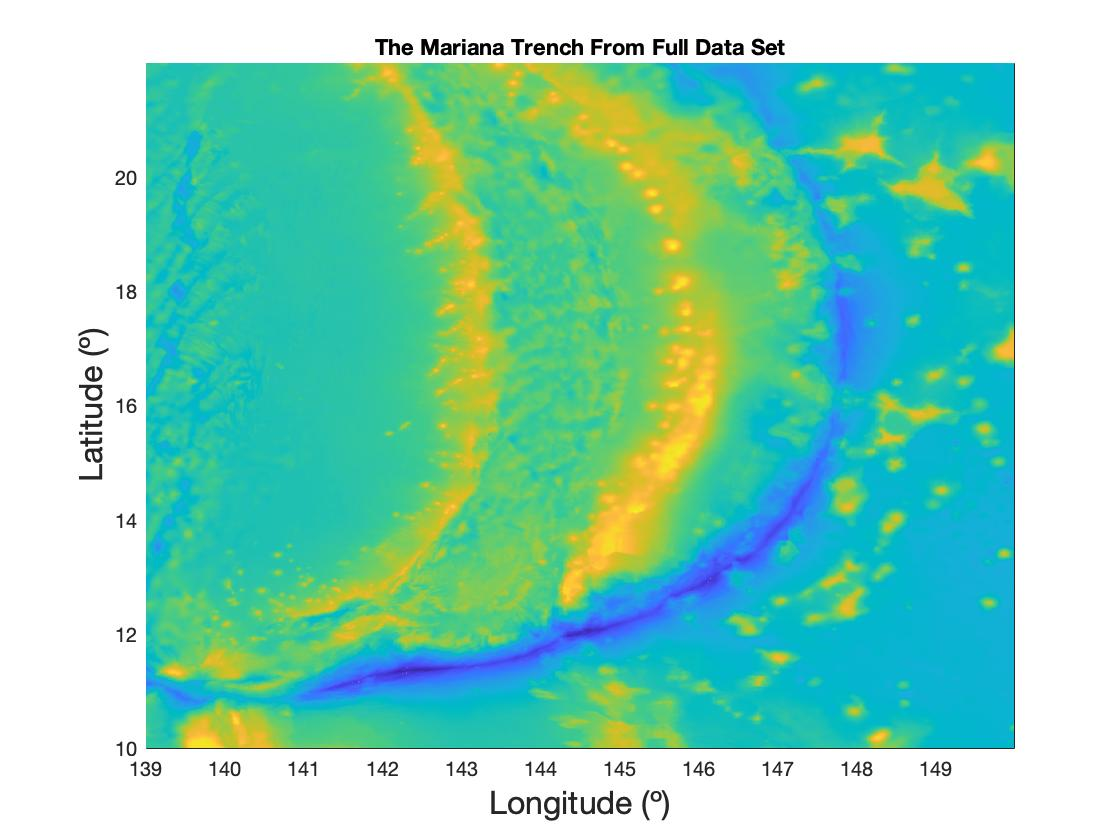
\includegraphics[width=0.45\textwidth]{./imgs/twoDFullDataSet.jpg}}}%
    \qquad 
    \subfloat[\centering $\text{ISVD} = \matr{U}\matr{\Sigma}\matr{V}^T$]
    {{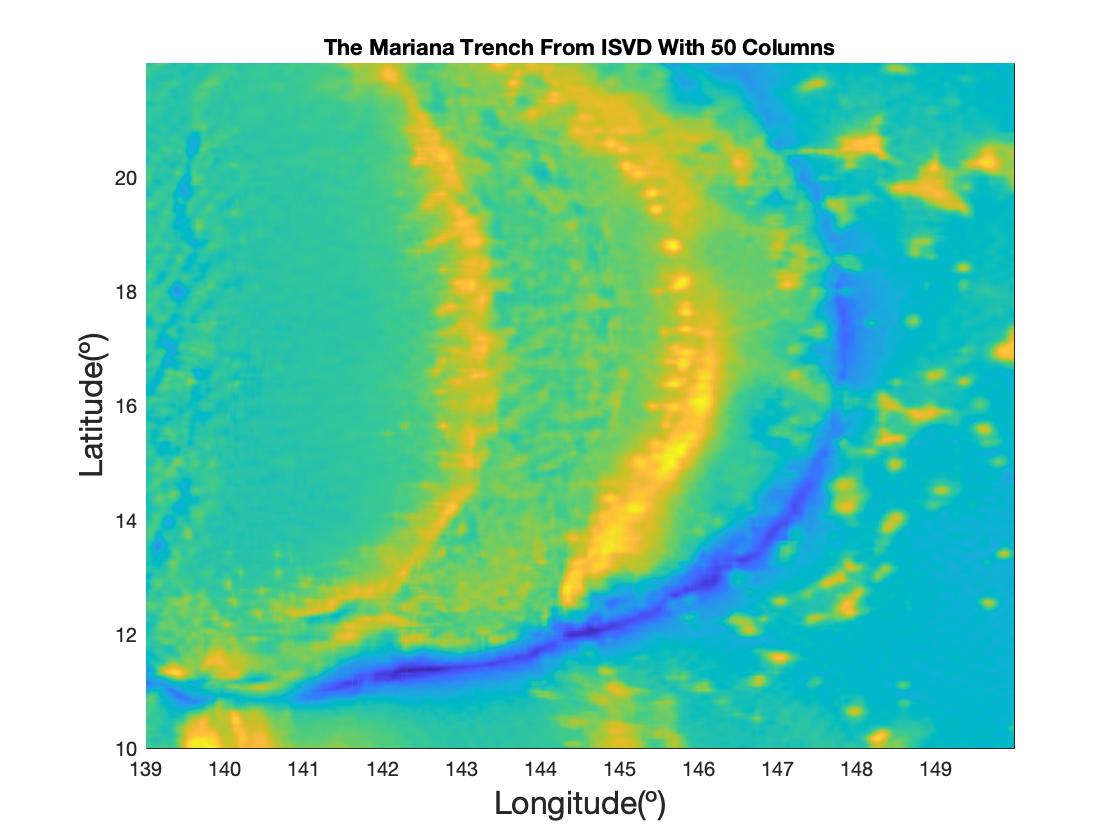
\includegraphics[width=0.45\textwidth]{./imgs/twoD50Col.jpg}}}%
    \caption{2D Plots of the Full Data Set and the ISVD Using 50 Eigenvalues}%
    \label{fig:502D}%
\end{figure}
Just looking at the 2D plots in \autoref{fig:502D}, we can see that the depth data looks basically the same, despite the reduction of values needed to store the data.
In fact, if we compare the average depth of the trench, using the same computation that was defined in Section \ref{sec:initInvest}, we see that the ISVD representation of the data has an average depth of 7.174 km compared to 7.205 km for the full data set, again showing how similar the ISVD is. Of course there is some slight difference, which can be seen in 3D plots in \autoref{fig:503D}. For example the few blue spikes that can be seen in the full data set graph are missing in the ISVD, and the ISVD is slightly smoother due to the compression. Still, the similarity between these plots shows that ISVD is a useful technique for reducing the number of values needed to represent a data set, while still maintaining the structure of the data.
\begin{figure}[H]
    \centering
    \subfloat[\centering $\mtrA$]
    {{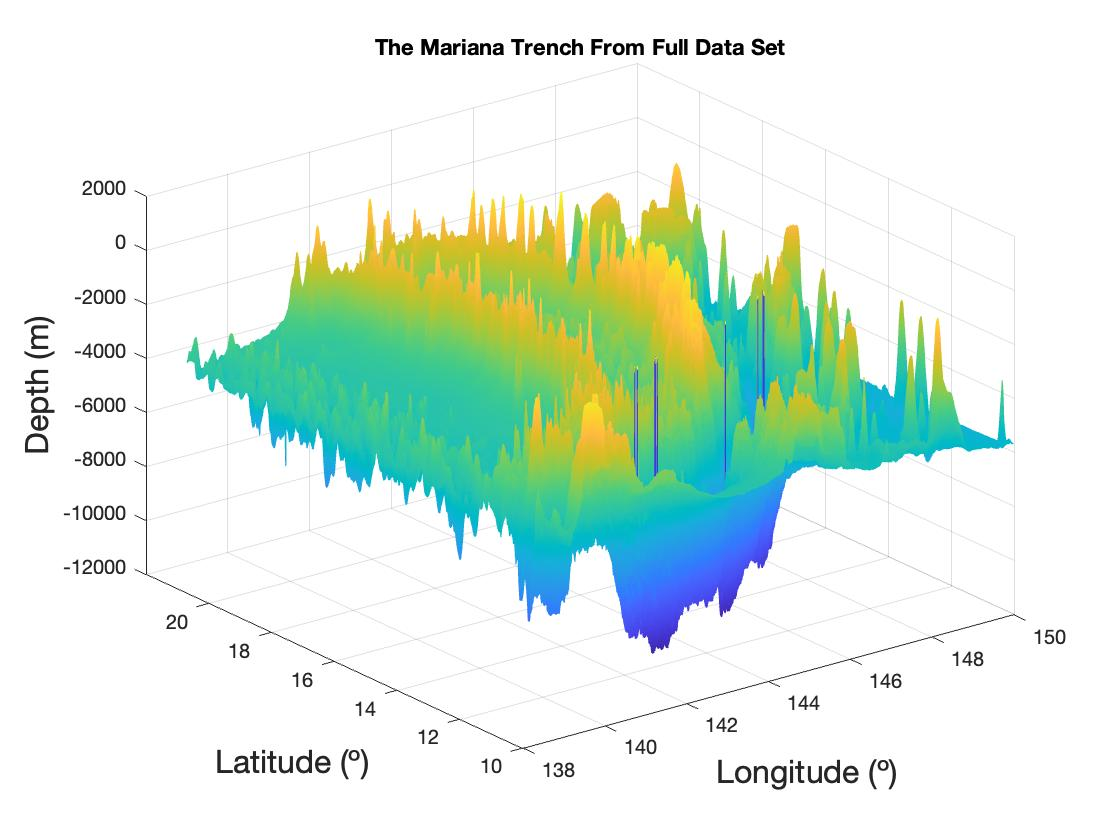
\includegraphics[width=0.45\textwidth]{./imgs/trueDataRendering.jpg}}}%
    \qquad
    \subfloat[\centering $\text{ISVD} = \matr{U}\matr{\Sigma}\matr{V}^T$]
    {{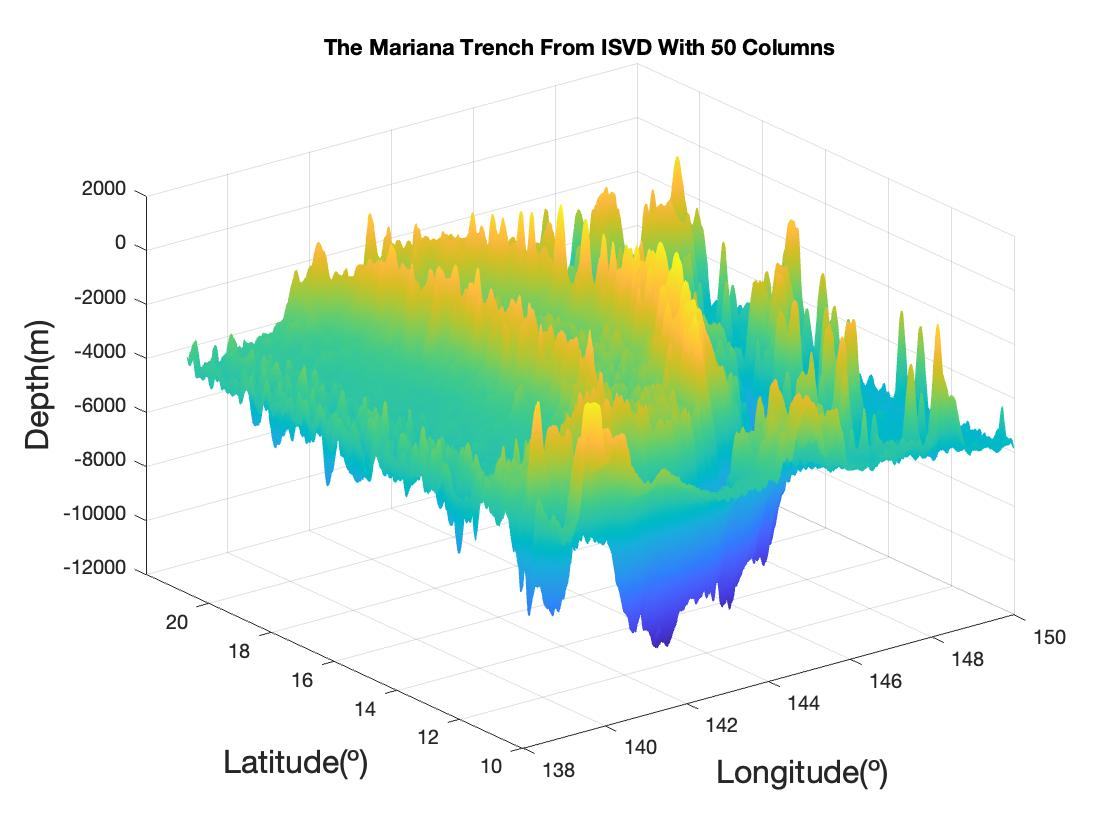
\includegraphics[width=0.45\textwidth]{./imgs/fiftyCol.jpg}}}%
    \caption{3D Plots of the Full Data Set and the ISVD Using 50 EigenValues}%
    \label{fig:503D}%
\end{figure}

%TODO: COMPUTE AVERAGE DEPTH FOR AT THE 50 column one, its ok if not the other ones

\subsection{Comparing the Full Data Set to ISVDs with a Varying Number of Eigenvalues}\label{sec:comparingISVDFAllGraphs}
Now that we have seen how ISVD with $50$ eigenvalues creates a good representation
of the Mariana Trench Data, we shall explore how the representation holds up as we vary the number of
eigenvalues used (and correspondingly reduce the sizes of $\mtrU,\mtrSig,\text{ and  }\mtrV$).
Doing this utilizing the methods explained in Section \ref{sec:allTogetherNow}, we can now investigate how changing the number of eigenvalues affects the fidelity of the data.

Comparing \autoref{fig:comparison3D} and \autoref{fig:503D}, we see that the data fidelity increases as the number of eigenvalues used in the ISVD goes up. In fact, looking at \autoref{fig:comparison3D}.d we can see that at 500 eigenvalues, the data is almost perfectly represented by the ISVD. This finding lines up with our intuition, as we would expect the data fidelity to increase as the compression rate
is decreased and more values are used to represent the data. 
\begin{figure}[H]
    \centering
    \subfloat[\centering Using $1$ Eigenvalue]
    {{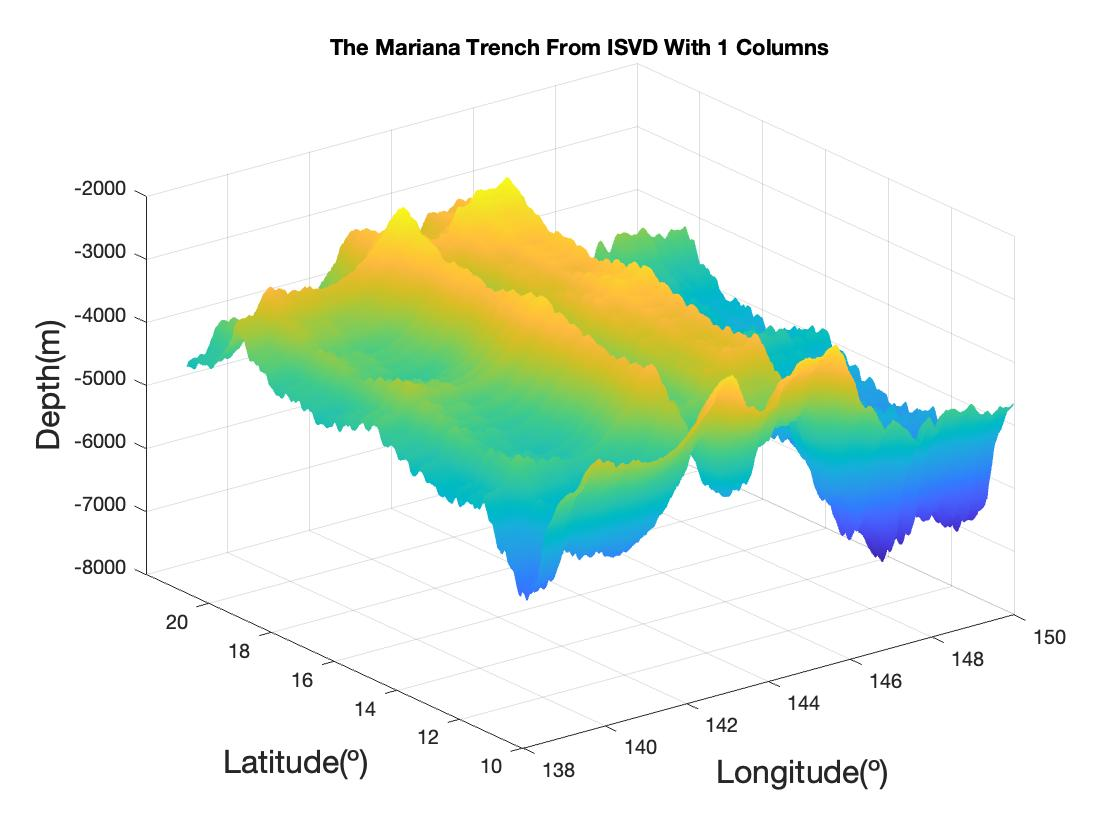
\includegraphics[width=0.45\textwidth]{./imgs/oneCol.jpg}}}%
    \qquad
    \subfloat[\centering Using $10$ Eigenvalues]
    {{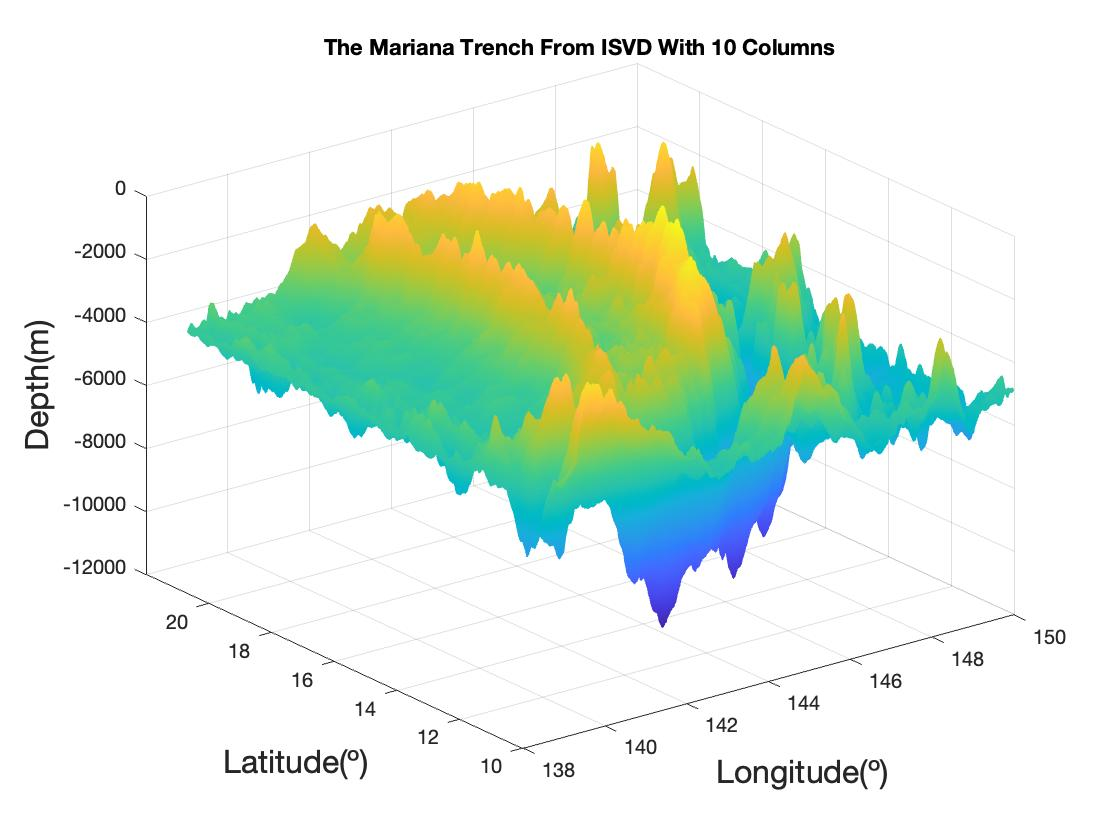
\includegraphics[width=0.45\textwidth]{./imgs/tenCol.jpg}}} \\
    \subfloat[\centering Using $100$ Eigenvalues]
    {{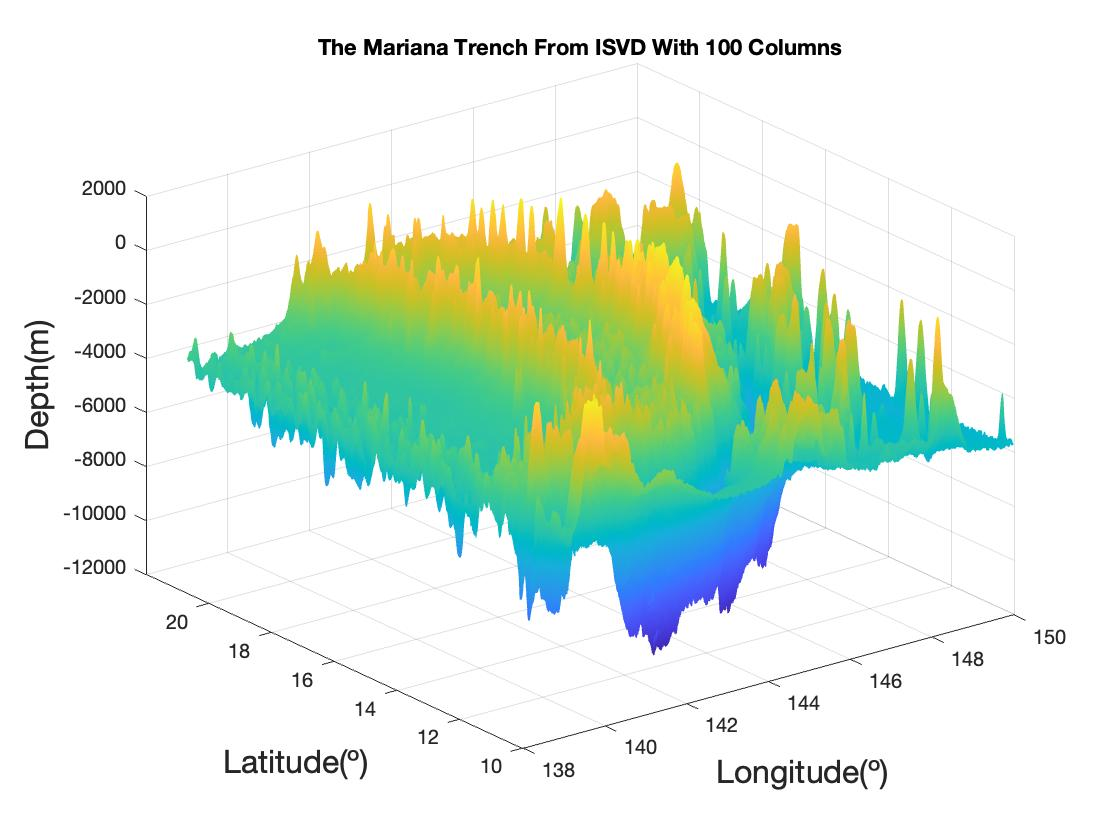
\includegraphics[width=0.45\textwidth]{./imgs/hundredCol.jpg}}}%
    \qquad
    \subfloat[\centering Using $500$ Eigenvalues]
    {{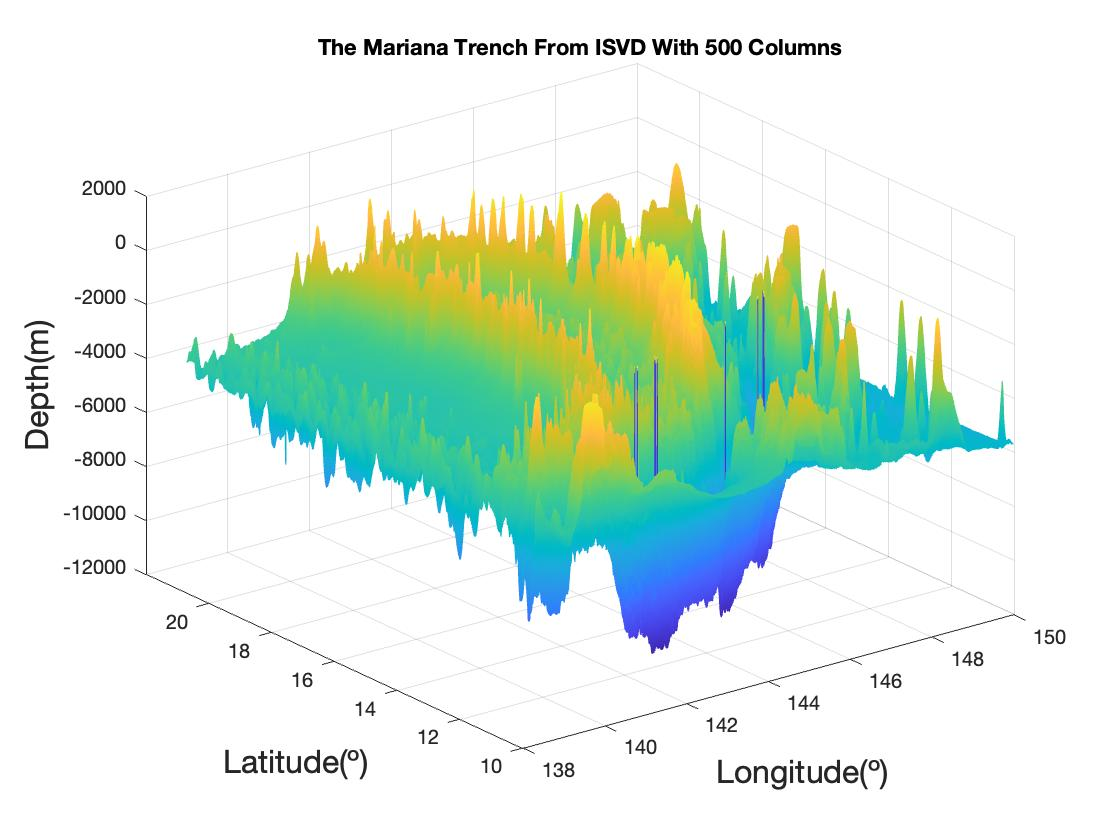
\includegraphics[width=0.45\textwidth]{./imgs/fiveHundCol.jpg}}}%
    \caption{3D Plots of ISVDs using Different Numbers of Eigenvalues for Comparison}%
    \label{fig:comparison3D}%
\end{figure}

\noindent
NOTE: 2D plots for this comparison were placed in the appendix for readability, see Section \ref{sec:isvdCompare2d} to view them.
